\documentclass{article}
\usepackage{tikz}

\usepackage{pgfplots}
\pgfplotsset{compat=1.15}
\usepackage{mathrsfs}
\usetikzlibrary{arrows, fit}


\begin{document}


\definecolor{zzttqq}{rgb}{0.6,0.2,0}
\definecolor{ududff}{rgb}{0.30196078431372547,0.30196078431372547,1}
% \begin{figure}
%     \centering
%         \begin{tikzpicture}
%         \end{tikzpicture}
%     \caption{gambar 1}
%     \label{fig:placeholder}
% \end{figure}

\tikz \draw (2,0) -- (3,1) ;

\vspace{2cm}

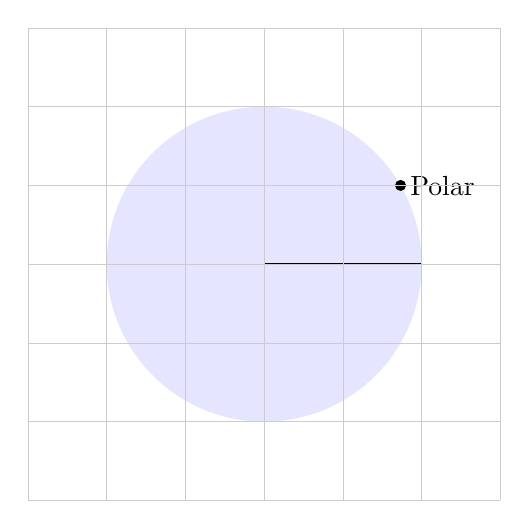
\begin{tikzpicture}
    \fill[blue!10](0,0) circle (2) ;
    \draw[thick](0,0) -- (2,0);
    \fill (30:2cm) circle (2pt) node[right] {Polar};
    % \fill (0:2cm) -- (30:2cm) -- (0,0) -- (0:2cm);
    \draw[help lines,gray!40] (-3,-3) grid (3,3);
\end{tikzpicture}

\vspace{2cm}

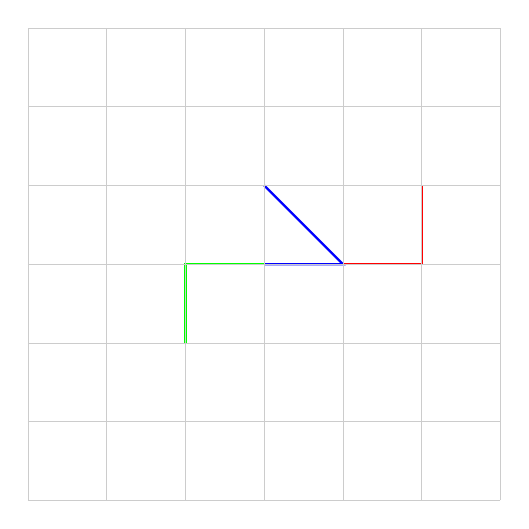
\begin{tikzpicture}
    \draw[red,thick] (0,0) -- (2,0) -- (2,1);
    \draw[blue,thick] (0,0) -- +(1,0) -- +(0,1);
    \draw[green, thick] (0,0) -- ++(-1,0) -- ++(0,-1);
    \draw[help lines,gray!40] (-3,-3) grid (3,3);
\end{tikzpicture}

\vspace{2cm}
\newpage

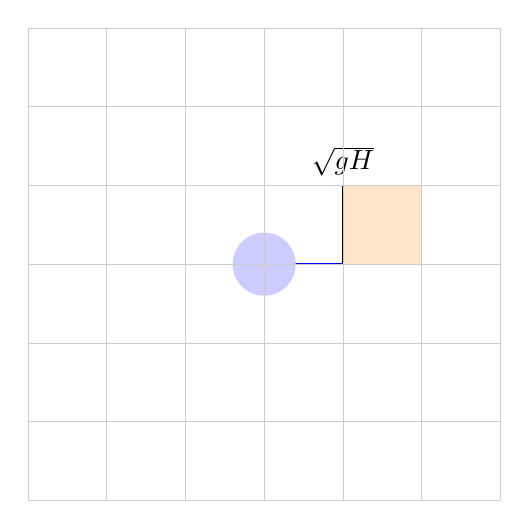
\begin{tikzpicture}
    \draw[blue,thick] (0,0) -- (2,0);
    \fill[blue!20] (0,0) circle (4mm);
    \filldraw[fill=orange!20,draw=black]
    (1,0) rectangle (2,1);
    \node[above] at (1,1) {$\sqrt{gH}$};
    % \filldraw[thick, red!50!blue, draw=green] (-3,-3) -- (-2,-2) -- (-1,-3) -- 
    % % \filldraw[thick, red!50!blue, draw=green] 
    % (0,-1) -- (1,0) -- (2,-1) -- cycle;
    
    \draw[help lines,gray!40] (-3,-3) grid (3,3);
\end{tikzpicture}


\newpage

\begin{figure}
    \centering
        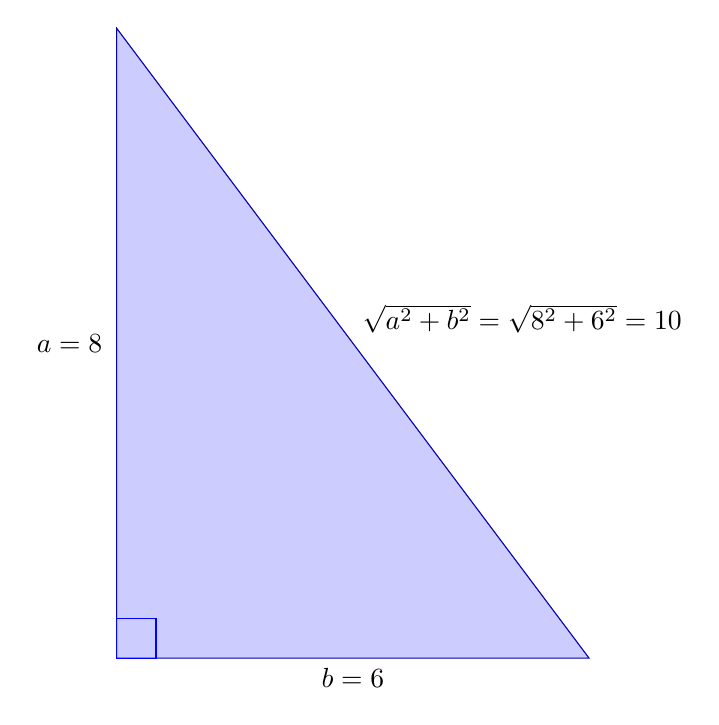
\begin{tikzpicture}

    \filldraw[draw=blue!70!black,fill=blue!20] (0,0) -- (0,8) -- (6,0) -- cycle;
    \draw[blue] (0,0) rectangle (.5,.5);
    \draw (0,4) node [left] {$a=8 \,$};
    \draw (3,0) node [below] {$b=6$};
    \draw (3,4) node [above right] {$\sqrt{a^2 + b^2} = \sqrt{8^2 + 6^2} = 10$};
    
\end{tikzpicture}

% \begin{tikzpicture}[line cap=round,line join=round,>=triangle 45,x=1cm,y=1cm]
% \begin{axis}[
% x=1cm,y=1cm,
% axis lines=middle,
% ymajorgrids=true,
% xmajorgrids=true,
% xmin=-10.68527099647973,
% xmax=23.533276331397282,
% ymin=-10.913759073516744,
% ymax=11.060289507488195,
% xtick={-10,-8,...,22},
% ytick={-10,-8,...,10},]
% \clip(-2,-1) rectangle (2,7);
% \fill[line width=2pt,color=zzttqq,fill=zzttqq,fill opacity=0.10000000149011612] (4.963300016120299,7.402181998049222) -- (-3.7247053187972496,-0.8285598981884658) -- (12.914603144275834,-0.8031563738173618) -- cycle;
% \draw [line width=2pt,color=zzttqq] (4.963300016120299,7.402181998049222)-- (-3.7247053187972496,-0.8285598981884658);
% \draw [line width=2pt,color=zzttqq] (-3.7247053187972496,-0.8285598981884658)-- (12.914603144275834,-0.8031563738173618);
% \draw [line width=2pt,color=zzttqq] (12.914603144275834,-0.8031563738173618)-- (4.963300016120299,7.402181998049222);
% \begin{scriptsize}
% \draw [fill=ududff] (4.963300016120299,7.402181998049222) circle (2.5pt);
% \draw [fill=ududff] (-3.7247053187972496,-0.8285598981884658) circle (2.5pt);
% \draw [fill=ududff] (12.914603144275834,-0.8031563738173618) circle (2.5pt);
% \end{scriptsize}
% \end{axis}
% \end{tikzpicture}
    \caption{Contoh aturan Phytagoras pada segitiga siku-siku}
    \label{fig:phytagoras}
\end{figure}


\newpage
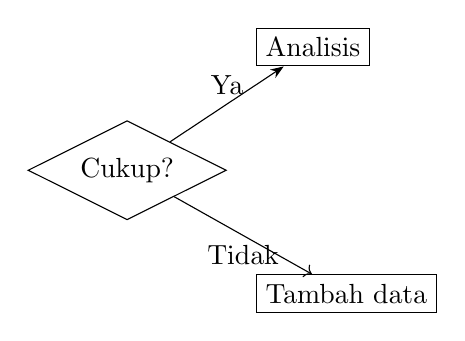
\begin{tikzpicture}
    % \node[draw] (a) at (0,0) {Masalah};
    % \node[draw] (b) at (3,0) {Metode};
    % \draw[->] (a.west) -- node[above] {dipelajari} (b.east);
    % \begin{scope}[xshift=2cm,rotate=45]
    % \draw (0,0) -- (1,0) -- (0,1);
    % \draw (0,1) -- (2,1);
    % \end{scope}
    
    % \foreach \x in {0,1,2,4,6,7,8} {
    %     \foreach \y in {0,1,2,3,4}
    %         {\fill (\x,\y) circle (2pt);}
    %     }
    
    
    % dengan pustaka fit:
    % \node[draw] (a) at (0,2){};
    % \node[draw] (b) at (1,2){};
    % \node[draw,fit=(a)(b),inner sep=4mm] {};

    \usetikzlibrary{shapes.geometric,positioning,arrows.meta}
    \node[draw,diamond,aspect=2] (cek) {Cukup?};
    \node[draw,above right=of cek] (ya) {Analisis};
    \node[draw,below right=of cek] (tidak) {Tambah data};
    \draw[-{Stealth}] (cek) -- node[above] {Ya} (ya);
    \draw[->] (cek) -- node[below] {Tidak} (tidak);
\end{tikzpicture}

\end{document}